\documentclass[12pt, titlepage]{article}

\usepackage{fullpage}
\usepackage[round]{natbib}
\usepackage{multirow}
\usepackage{booktabs}
\usepackage{tabularx}
\usepackage{graphicx}
\usepackage{float}
\usepackage{hyperref}
\hypersetup{
    colorlinks,
    citecolor=blue,
    filecolor=black,
    linkcolor=red,
    urlcolor=blue
}

%% Comments

\usepackage{color}

\newif\ifcomments\commentstrue %displays comments
%\newif\ifcomments\commentsfalse %so that comments do not display

\ifcomments
\newcommand{\authornote}[3]{\textcolor{#1}{[#3 ---#2]}}
\newcommand{\todo}[1]{\textcolor{red}{[TODO: #1]}}
\else
\newcommand{\authornote}[3]{}
\newcommand{\todo}[1]{}
\fi

\newcommand{\wss}[1]{\authornote{blue}{SS}{#1}} 
\newcommand{\plt}[1]{\authornote{magenta}{TPLT}{#1}} %For explanation of the template
\newcommand{\an}[1]{\authornote{cyan}{Author}{#1}}

%% Common Parts

\newcommand{\progname}{Mechtronics Enigeering} % PUT YOUR PROGRAM NAME HERE
\newcommand{\authname}{Team 32, Wingman
\\ Edward He
\\ Erping Zhang
\\ Guangwei Tang
\\ Peng Cui
\\ Peihua Jin } % AUTHOR NAMES                  

\usepackage{hyperref}
    \hypersetup{colorlinks=true, linkcolor=blue, citecolor=blue, filecolor=blue,
                urlcolor=blue, unicode=false}
    \urlstyle{same}
                                


\newcounter{acnum}
\newcommand{\actheacnum}{AC\theacnum}
\newcommand{\acref}[1]{AC\ref{#1}}

\newcounter{ucnum}
\newcommand{\uctheucnum}{UC\theucnum}
\newcommand{\uref}[1]{UC\ref{#1}}

\newcounter{mnum}
\newcommand{\mthemnum}{M\themnum}
\newcommand{\mref}[1]{M\ref{#1}}

\begin{document}

\title{Module Guide for \progname{}} 
\author{\authname}
\date{\today}

\maketitle

\pagenumbering{roman}

\section{Revision History}

\begin{tabularx}{\textwidth}{p{3cm}p{2cm}X}
\toprule {\bf Date} & {\bf Version} & {\bf Notes}\\
\midrule
Date 1 & 1.0 & Notes\\
Date 2 & 1.1 & Notes\\
\bottomrule
\end{tabularx}

\newpage

\section{Reference Material}

This section records information for easy reference.

\subsection{Abbreviations and Acronyms}

\renewcommand{\arraystretch}{1.2}
\begin{tabular}{l l} 
  \toprule		
  \textbf{symbol} & \textbf{description}\\
  \midrule 
  DAG & Directed Acyclic Graph \\
  LC & Likely Change\\
  M & Module \\
  MG & Module Guide \\
  OS & Operating System \\
  R & Requirement\\
  SC & Scientific Computing \\
  SRS & Software Requirements Specification\\
  \progname & Explanation of program name\\
  UC & Unlikely Change \\
  \wss{etc.} & \wss{...}\\
  \bottomrule
\end{tabular}\\

\newpage

\tableofcontents

\listoftables

\listoffigures

\newpage

\pagenumbering{arabic}

\section{Introduction}

Decomposing a system into modules is a commonly accepted approach to developing
software.  A module is a work assignment for a programmer or programming
team~\citep{ParnasEtAl1984}.  We advocate a decomposition
based on the principle of information hiding~\citep{Parnas1972a}.  This
principle supports design for change, because the ``secrets'' that each module
hides represent likely future changes.  Design for change is valuable in SC,
where modifications are frequent, especially during initial development as the
solution space is explored.  

Our design follows the rules layed out by \citet{ParnasEtAl1984}, as follows:
\begin{itemize}
\item System details that are likely to change independently should be the
  secrets of separate modules.
\item Each data structure is implemented in only one module.
\item Any other program that requires information stored in a module's data
  structures must obtain it by calling access programs belonging to that module.
\end{itemize}

After completing the first stage of the design, the Software Requirements
Specification (SRS), the Module Guide (MG) is developed~\citep{ParnasEtAl1984}. The MG
specifies the modular structure of the system and is intended to allow both
designers and maintainers to easily identify the parts of the software.  The
potential readers of this document are as follows:

\begin{itemize}
\item New project members: This document can be a guide for a new project member
  to easily understand the overall structure and quickly find the
  relevant modules they are searching for.
\item Maintainers: The hierarchical structure of the module guide improves the
  maintainers' understanding when they need to make changes to the system. It is
  important for a maintainer to update the relevant sections of the document
  after changes have been made.
\item Designers: Once the module guide has been written, it can be used to
  check for consistency, feasibility and flexibility. Designers can verify the
  system in various ways, such as consistency among modules, feasibility of the
  decomposition, and flexibility of the design.
\end{itemize}

The rest of the document is organized as follows. Section 4 lists the likely and unlikely changes of the software requirements. Section 5 gives a detailed description of the
modules. Section 6 describes the use relation between modules. Section 7 specifies the connections between the software requirements and the modules and includes two traceability matrices. One checks
the completeness of the design against the requirements provided in the SRS. The
other shows the relation between anticipated changes and the modules. 

\section{Likely and Unlikely Changes} \label{SecChange}

This section lists possible changes to the system. According to the likeliness
of the change, the possible changes are classified into two
categories. Likely changes are listed in Section \ref{SecLchange}, and
unlikely changes are listed in Section \ref{SecUchange}.

\subsection{Likely Changes} \label{SecLchange}

Likely changes are the source of the information that is to be hidden
inside the modules. Ideally, changing one of the likely changes will only
require changing the one module that hides the associated decision. The approach
adapted here is called design for change.\\\\
\textbf{LC1:} The camera may get upgraded and replaced with the one with higher resolution to achieve more accurate images.\\
\textbf{Rationale:} To ensure that Image Processing Module could collect clear information with high resolution.\\\\
\textbf{LC2:} The security of user’s private account will be strengthened. \\
\textbf{Rationale:} It is necessary to safely protect the private information of the users’.\\\\
\textbf{LC3:} The specific
hardware on which the software is running.\\\\
\textbf{LC4:} The algorithm of Image Processing Module and Information Storage Module might be optimized.\\
\textbf{Rationale:} To accurately execute the task and efficiently track the missing item.\\\\
\textbf{LC5:} Any one except for the users is not allowed to access the any file that stores the information about the objects in the room.\\\\
\textbf{LC6:} The device is supposed to work in only indoor space.\\
\textbf{Rationale:} To ensure that the system is able to adapt multiple environment.\\



\subsection{Unlikely Changes}  \label{SecUchange}

The module design should be as general as possible. However, a general system is
more complex. Sometimes this complexity is not necessary. Fixing some design
decisions at the system architecture stage can simplify the software design. If
these decision should later need to be changed, then many parts of the design
will potentially need to be modified. Hence, it is not intended that these
decisions will be changed.\\\\
\textbf{UC1:} The maintenance for the device should be done by the developers.\\\\
\textbf{UC2:} The performance of the product should not violate the laws that protect the privacy of the user. \\
\textbf{Rationale:} To ensure that the private information of the users’is safely protected.\\\\
\textbf{UC3:} The device is supported by any computers supports both C and python programming languages.\\\\
\textbf{UC4:} The device should be easy to installed in the room.\\
\textbf{Rationale:} To satisfy the convenience of the installation of the device.\\\\
\textbf{UC5:} The device should not have exposed internal electronic wiring.\\\\
\textbf{UC6:} The base of the device should be strong enough without falling from the floor.\\
\textbf{Rationale:} To ensure that the base of the system is stable enough to avoid any accidents\\


\section{Secret of Each Module} 
\subsection{Software Modules}
\subsubsection{Login Module}
\begin{description}
\item[Secrets:]The data structure and unit used to login in to the personal account.
\item[Services:]This module provides the interface between the user and the application. So, the system can use it to display personal account.
\item[Implemented By:] Python
\end{description}
\subsubsection{Information Storage Module}
\begin{description}
\item[Secrets:]The unit used to storage data and information
hardware.
\item[Services:]Provides with a storage platform used by the rest of the system. This module protects the data and store the information and picture of the recorded items. Once the object detection is captured by the Image Processing Module, the camera will take a photo and store in the local file. Therefore, the system can use it to display and fetch out the desired information.
\item[Implemented By:] Python
\end{description}
\subsubsection{Image Processing Module}
\paragraph{5.1.3.1	 Object Detection Module}
\begin{description}
\item[Secrets:]The data structure and algorithm used to implement the image processing and compare the image differences.
\item[Services:]This module serves as a tool to capture the object movement. In addition, it provides with the function for the comparison of different positions. So, the system can use it to process the required basic operation.
\item[Implemented By:] Python
\end{description}
\paragraph{5.1.3.2	 Human Detection Module}
\begin{description}
\item[Secrets:]The data structure and algorithm used to implement the image processing and capture the movement of human.
\item[Services:]This module serves as a tool to capture the human movement. So, the system can use it to process the required basic operation.
\item[Implemented By:] Python
\end{description}

\subsubsection{Information Extraction Module}
\begin{description}
\item[Secrets:]The module unit implemented to display specific information and attribute of the desired object.
\item[Services:]Serves as an information extraction system. This module cooperates with the Information Storage Module to output the required information which depends on the attributes chosen by the user. Consequently, the system can use it to display outputs according to various variables determined by the user.
\item[Implemented By:] Python
\end{description}
\subsubsection{Communication Port 1 Module}
\begin{description}
\item[Secrets:]This module unit is used to connect the software data with the hardware module through sending the USB signal, which is considered as a serial communication system.
\item[Services:]Serves as a connection bridge between the hardware and software module in the system. This module works along with the Communication Port 2 Module to deal with the data transmission through sending command from the software end to the hardware end. Thus, the system can use it to transmit and receive data and signals from the hardware module unit.
\item[Implemented By:] Python
\end{description}

\subsection{Hardware Module}

\subsubsection{Communication Port 2 Module}
\begin{description}
\item[Secrets:] This module unit is used to communicate the data and signal with the software module through reading the USB signal, which is defined as a serial communication system.
\item[Services:]Behaves as a link between the hardware and software module in the system. This module works along with the Communication Port 1 Module to receive the data transmitted from the software end. Therefore, the system can use it to receive data and signals from the software module unit and also send the data to the software system.
\item[Implemented By:] Python
\end{description}
\subsubsection{Motor Control Module}
\begin{description}
\item[Secrets:]The hardware module designed to implement the control of step motor, including the two-dimension speed control, human movement capture.
\item[Services:]The module serves as a unit to control the rotatory angular velocity of the motor, which is implemented with a closed-loop control as the controller of the angular speed of step motor. So, the system can use it to proceed the desired basic operation.
\item[Implemented By:] Python
\end{description}


\subsection{Module Summary}
This section provides an overview of the module design. Modules are summarized
in a hierarchy decomposed by secrets in Table \ref{TableMS}. The modules listed
below, which are leaves in the hierarchy tree, are the modules that will
actually be implemented.
\begin{table}[H]
\begin{tabularx}{\textwidth}{XX}
  \toprule		
  \textbf{symbol} & \textbf{description}\\
  \midrule 
  M1 & Login Module \\
  M2 & Information Storage Module \\
  M3 & Image Processing Module \\
  M4 & Information Extraction Module \\
  M5 & Communication Port 1 Module \\
  M6 & Communication Port 2 Module \\
  M7 & Motor Control Module \\
  \bottomrule
\end{tabularx}
\caption{Module Summary}
\label{TableMS}
\end{table}

\begin{table}[H]
\begin{tabularx}{\textwidth}{XXX}
  \toprule		
  \textbf{Assigned Task} & \textbf{Designer} & \textbf{Deadline}\\
  \midrule 
  M1 & Cui, Peng & 1.31\\
  M2 & He, Edward and Jin, Peihua & 1.31\\
  M3 & He, Edward and Jin, Peihua and Zhang, Erping & 1.31\\
  M4 & Jin, Peihua and Cui, Peng & 1.31\\
  M5 & Cui, Peng & 1.31\\
  M6 & Tang, Guangwei & 1.31\\
  M7 & Zhang, Erping & 1.31\\
  Phase 1 & All & 2.10\\
  Phase 2 & All & 2.30\\
  Final & All & 3.15\\
  \bottomrule
\end{tabularx}
\caption{Timeline}
\label{TableTL}
\end{table}


\section{Relationship Between Modules} 

In this section, the uses hierarchy between modules is
provided. \citet{Parnas1978} said of two programs A and B that A {\em uses} B if
correct execution of B may be necessary for A to complete the task described in
its specification. That is, A {\em uses} B if there exist situations in which
the correct functioning of A depends upon the availability of a correct
implementation of B.  Figure \ref{FigUH} illustrates the use relation between
the modules. It can be seen that the graph is a directed acyclic graph
(DAG). Each level of the hierarchy offers a testable and usable subset of the
system, and modules in the higher level of the hierarchy are essentially simpler
because they use modules from the lower levels.\\
\\
In summary, the user has to login into the account through Login Module M1. Then, he or she is expected to look for the desired item using Information Extraction Module M4 with multiple searching keys. The information and data are stored in Information Storage Module M2 and progressed by Image Processing Module M3. In addition, the data transmission between the hardware-end and the software-end is connected with Communication Port 1 Module M5 and Communication Port 2 Module M6. The motor is controlled and operated by Motor Control Module M7.


\begin{figure}[H]
\centering
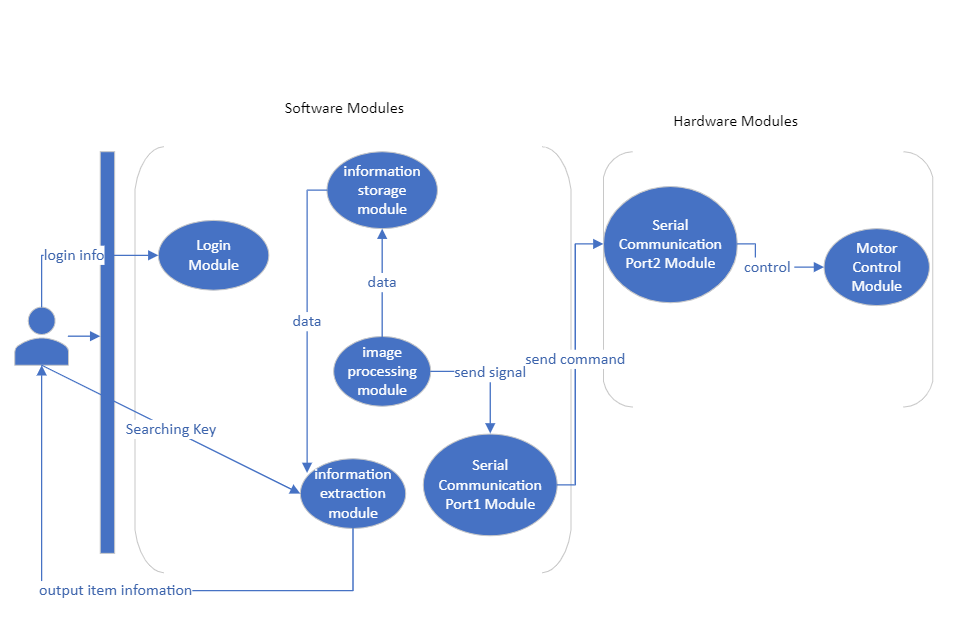
\includegraphics[width=1\textwidth]{UsesHierarchy.png}
\caption{Use hierarchy among modules}
\label{FigUH}
\end{figure}


\section{Relationship Between Modules and SRS}
This part specifies the connections between the software requirements and the modules.\\\\
\textbf{IPR1:} Image Processing Module M3 is able to identify human's body.\\\\
\textbf{IPR2:} Image Processing Module M3 could identify human's hand.\\\\
\textbf{IPR3:} Information Storage Module M2 and Image Processing Module M3 should be able to identify all the small items being exposed to the camera.\\\\
\textbf{IPR4:} Information Storage Module M2, Image Processing Module M3, Information Extraction Module M4 should take a photo once the change of the location of an item is captured.\\\\
\textbf{IPR5:} Information Storage Module M2, Image Processing Module M3, Information Extraction Module M4 should be able to differentiate one item from another items which are identified by the system through 3 main parameters, item\_shape, item\_color and item\_size.\\\\
\textbf{IPR6:} Information Storage Module M2, Information Extraction Module M4 must be able to store all the photos into a file, and indicate the time when it was taken.\\\\
\textbf{IPR7:} Information Storage Module M2, Information Extraction Module M4 must be able to name each item with a unique ID.\\\\
\textbf{IPR8:} Information Storage Module M2 should be able to arrange the photos stored in the file in ascending or descending order according to the time it was taken.\\\\
\textbf{IPR9:} Information Storage Module M2 should be able to arrange the photos stored in the file in ascending or descending order according to their IDs.\\\\
\textbf{UIR1:} Information Storage Module M2 should be able to let user to choose whether to highlight a certain item or not.\\\\
\textbf{UIR2:} Information Storage Module M2, Information Extraction Module M4 should be able to let user to switch the ordering method.\\\\
\textbf{UIR3:} Login Module M1, Information Storage Module M2, Image Processing Module M3, Information Extraction Module M4 must be able to notify the user when the WI-FI signal is weak or unstable.\\\\
\textbf{UIR4:} Login Module M1, and Information Storage Module M2 must be able to allow the user to view the system's status at any given point in time.\\

This section shows two traceability matrices: between the modules and the
requirements and between the modules and the anticipated changes.

% the table should use mref, the requirements should be named, use something
% like fref
\begin{table}[H]
\centering
\begin{tabular}{p{0.2\textwidth} p{0.6\textwidth}}
\toprule
\textbf{Req.} & \textbf{Modules}\\
\midrule
IPR1 & M3\\
IPR2 & M3\\
IPR3 & M2, M3\\
IPR4 & M2, M3, M4\\
IPR5 & M2, M3, M4\\
IPR6 & M2, M4\\
IPR7 & M2, M4\\
IPR8 & M2\\
IPR9 & M2\\
UIR1 & M2\\
UIR2 & M2, M4\\
UIR3 & M1, M2, M3, M4\\
UIR4 & M1, M2\\
\bottomrule
\end{tabular}
\caption{Trace Between Requirements and Modules}
\label{TblRT}
\end{table}

\begin{table}[H]
\centering
\begin{tabular}{p{0.2\textwidth} p{0.6\textwidth}}
\toprule
\textbf{LC} & \textbf{Modules}\\
\midrule
LC1 & M6, M7\\
LC2 & M1 ,M2\\
LC3 & M6\\
LC4 & M2, M3\\
LC5 & M1\\
LC6 & -\\
\bottomrule
\end{tabular}
\caption{Trace Between Likely Changes and Modules}
\label{TblACT}
\end{table}



%\section*{References}

\bibliographystyle {plainnat}
\bibliography{../../../refs/References}


\end{document}
